% Options for packages loaded elsewhere
\PassOptionsToPackage{unicode,linktoc=all}{hyperref}
\PassOptionsToPackage{hyphens}{url}
\PassOptionsToPackage{dvipsnames,svgnames,x11names}{xcolor}
%
\documentclass[
  a4paper,
]{article}
\usepackage{amsmath,amssymb}
\usepackage{iftex}
\ifPDFTeX
  \usepackage[T1]{fontenc}
  \usepackage[utf8]{inputenc}
  \usepackage{textcomp} % provide euro and other symbols
\else % if luatex or xetex
  \usepackage{unicode-math} % this also loads fontspec
  \defaultfontfeatures{Scale=MatchLowercase}
  \defaultfontfeatures[\rmfamily]{Ligatures=TeX,Scale=1}
\fi
\usepackage{lmodern}
\ifPDFTeX\else
  % xetex/luatex font selection
\fi
% Use upquote if available, for straight quotes in verbatim environments
\IfFileExists{upquote.sty}{\usepackage{upquote}}{}
\IfFileExists{microtype.sty}{% use microtype if available
  \usepackage[]{microtype}
  \UseMicrotypeSet[protrusion]{basicmath} % disable protrusion for tt fonts
}{}
\makeatletter
\@ifundefined{KOMAClassName}{% if non-KOMA class
  \IfFileExists{parskip.sty}{%
    \usepackage{parskip}
  }{% else
    \setlength{\parindent}{0pt}
    \setlength{\parskip}{6pt plus 2pt minus 1pt}}
}{% if KOMA class
  \KOMAoptions{parskip=half}}
\makeatother
\usepackage{xcolor}
\usepackage[margin=25mm]{geometry}
\usepackage{longtable,booktabs,array}
\usepackage{calc} % for calculating minipage widths
% Correct order of tables after \paragraph or \subparagraph
\usepackage{etoolbox}
\makeatletter
\patchcmd\longtable{\par}{\if@noskipsec\mbox{}\fi\par}{}{}
\makeatother
% Allow footnotes in longtable head/foot
\IfFileExists{footnotehyper.sty}{\usepackage{footnotehyper}}{\usepackage{footnote}}
\makesavenoteenv{longtable}
\usepackage{graphicx}
\makeatletter
\def\maxwidth{\ifdim\Gin@nat@width>\linewidth\linewidth\else\Gin@nat@width\fi}
\def\maxheight{\ifdim\Gin@nat@height>\textheight\textheight\else\Gin@nat@height\fi}
\makeatother
% Scale images if necessary, so that they will not overflow the page
% margins by default, and it is still possible to overwrite the defaults
% using explicit options in \includegraphics[width, height, ...]{}
\setkeys{Gin}{width=\maxwidth,height=\maxheight,keepaspectratio}
% Set default figure placement to htbp
\makeatletter
\def\fps@figure{htbp}
\makeatother
\setlength{\emergencystretch}{3em} % prevent overfull lines
\providecommand{\tightlist}{%
  \setlength{\itemsep}{0pt}\setlength{\parskip}{0pt}}
\setcounter{secnumdepth}{-\maxdimen} % remove section numbering
% definitions for citeproc citations
\NewDocumentCommand\citeproctext{}{}
\NewDocumentCommand\citeproc{mm}{%
  \begingroup\def\citeproctext{#2}\cite{#1}\endgroup}
\makeatletter
 % allow citations to break across lines
 \let\@cite@ofmt\@firstofone
 % avoid brackets around text for \cite:
 \def\@biblabel#1{}
 \def\@cite#1#2{{#1\if@tempswa , #2\fi}}
\makeatother
\newlength{\cslhangindent}
\setlength{\cslhangindent}{1.5em}
\newlength{\csllabelwidth}
\setlength{\csllabelwidth}{3em}
\newenvironment{CSLReferences}[2] % #1 hanging-indent, #2 entry-spacing
 {\begin{list}{}{%
  \setlength{\itemindent}{0pt}
  \setlength{\leftmargin}{0pt}
  \setlength{\parsep}{0pt}
  % turn on hanging indent if param 1 is 1
  \ifodd #1
   \setlength{\leftmargin}{\cslhangindent}
   \setlength{\itemindent}{-1\cslhangindent}
  \fi
  % set entry spacing
  \setlength{\itemsep}{#2\baselineskip}}}
 {\end{list}}
\usepackage{calc}
\newcommand{\CSLBlock}[1]{\hfill\break#1\hfill\break}
\newcommand{\CSLLeftMargin}[1]{\parbox[t]{\csllabelwidth}{\strut#1\strut}}
\newcommand{\CSLRightInline}[1]{\parbox[t]{\linewidth - \csllabelwidth}{\strut#1\strut}}
\newcommand{\CSLIndent}[1]{\hspace{\cslhangindent}#1}
\ifLuaTeX
\usepackage[bidi=basic]{babel}
\else
\usepackage[bidi=default]{babel}
\fi
\babelprovide[main,import]{british}
% get rid of language-specific shorthands (see #6817):
\let\LanguageShortHands\languageshorthands
\def\languageshorthands#1{}
% $HOME/.pandoc/defaults/latex-header-includes.tex
% Common header includes for both lualatex and xelatex engines.
%
% Preliminaries
%
% \PassOptionsToPackage{rgb,dvipsnames,svgnames}{xcolor}
% \PassOptionsToPackage{main=british}{babel}
\PassOptionsToPackage{english}{selnolig}
\AtBeginEnvironment{quote}{\small}
\AtBeginEnvironment{quotation}{\small}
\AtBeginEnvironment{longtable}{\centering}
%
% Packages that are useful to include
%
\usepackage{graphicx}
\usepackage{subcaption}
\usepackage[inkscapeversion=auto]{svg}
\usepackage[defaultlines=4,all]{nowidow}
\usepackage{etoolbox}
\usepackage{fontsize}
\usepackage{newunicodechar}
\usepackage{pdflscape}
\usepackage{fnpct}
\usepackage{parskip}
  \setlength{\parindent}{0pt}
\usepackage[style=american]{csquotes}
% \usepackage{setspace} Use the <fontname-plus.tex> files for setspace
%
\usepackage{hyperref} % cleveref must come AFTER hyperref
\usepackage[capitalize,noabbrev]{cleveref} % Must come after hyperref
\let\longdivision\relax
\usepackage{longdivision}
\newcommand{\dd}{\ensuremath{mathrm d}}
% noto-plus.tex
% Font-setting header file for use with Pandoc Markdown
% to generate PDF via LuaLaTeX.
% The main font is Noto Serif.
% Other main fonts are also available in appropriately named file.
\usepackage{fontspec}
\usepackage{setspace}
\setstretch{1.3}
%
\defaultfontfeatures{Ligatures=TeX,Scale=MatchLowercase,Renderer=Node} % at the start always
%
% For English
% See also https://tex.stackexchange.com/questions/574047/lualatex-amsthm-polyglossia-charissil-error
% We use Node as Renderer for the Latin Font and Greek Font and HarfBuzz as renderer ofr Indic fonts.
%
\babelfont{rm}[Script=Latin,Scale=1]{NotoSerif}% Config is at $HOME/texmf/tex/latex/NotoSerif.fontspec
\babelfont{sf}[Script=Latin]{SourceSansPro}% Config is at $HOME/texmf/tex/latex/SourceSansPro.fontspec
\babelfont{tt}[Script=Latin]{FiraMono}% Config is at $HOME/texmf/tex/latex/FiraMono.fontspec
%
% Sanskrit, Tamil, and Greek fonts
%
\babelprovide[import, onchar=ids fonts]{sanskrit}
\babelprovide[import, onchar=ids fonts]{tamil}
\babelprovide[import, onchar=ids fonts]{greek}
%
\babelfont[sanskrit]{rm}[Scale=1.1,Renderer=HarfBuzz,Script=Devanagari]{NotoSerifDevanagari}
\babelfont[sanskrit]{sf}[Scale=1.1,Renderer=HarfBuzz,Script=Devanagari]{NotoSansDevanagari}
\babelfont[tamil]{rm}[Renderer=HarfBuzz,Script=Tamil]{NotoSerifTamil}
\babelfont[tamil]{sf}[Renderer=HarfBuzz,Script=Tamil]{NotoSansTamil}
\babelfont[greek]{rm}[Script=Greek]{GentiumBookPlus}
%
% Math font
%
\usepackage{unicode-math} % seems not to hurt % fallabck
\setmathfont[bold-style=TeX]{STIX Two Math}
\usepackage{amsmath}
\usepackage{esdiff} % for derivative symbols
% \renewcommand{\mathbf}{\symbf}
%
%
% Other fonts
%
\newfontfamily{\emojifont}{Symbola}
%

\usepackage{titling}
\usepackage{fancyhdr}
    \pagestyle{fancy}
    \fancyhead{}
    \fancyfoot{}
    \renewcommand{\headrulewidth}{0.2pt}
    \renewcommand{\footrulewidth}{0.2pt}
    \fancyhead[LO,RE]{\scshape\thetitle}
    \fancyfoot[CO,CE]{\footnotesize Copyright © 2006\textendash\the\year, R (Chandra) Chandrasekhar}
    \fancyfoot[RE,RO]{\thepage}
%
\usepackage{newunicodechar}
\newunicodechar{√}{\textsf{√}}
\usepackage {caption}
    \captionsetup{font={sf,stretch=1.4}}
\ifLuaTeX
  \usepackage{selnolig}  % disable illegal ligatures
\fi
\IfFileExists{bookmark.sty}{\usepackage{bookmark}}{\usepackage{hyperref}}
\IfFileExists{xurl.sty}{\usepackage{xurl}}{} % add URL line breaks if available
\urlstyle{sf}
\hypersetup{
  pdftitle={Same Action: Four Castes},
  pdfauthor={R (Chandra) Chandrasekhar},
  pdflang={en-GB},
  colorlinks=true,
  linkcolor={DarkGreen},
  filecolor={Purple},
  citecolor={Teal},
  urlcolor={Maroon},
  pdfcreator={LaTeX via pandoc}}

\title{Same Action: Four Castes}
\author{R (Chandra) Chandrasekhar}
\date{2008-10-24 | 2024-08-02}

\begin{document}
\maketitle

\thispagestyle{empty}


\begin{quote}
This blog was originally penned on 24 October 2008. It is one among many
dozen blogs that have not been released publicly on the Web. I will be
gradually refreshing and releasing all those unpublished blogs on this
website. They are generally short and tightly focused pieces of writing,
readable in a few minutes. I have retained the original contextual
immediacy and topical relevance, where possible. I have used the
\href{https://en.wikipedia.org/wiki/International_Alphabet_of_Sanskrit_Transliteration}{IAST}
transliteration scheme for the Sanskrit terms; see the link for the
correct pronunciation.

The upshot of this blog is that caste is spiritual in nature, and that
all individuals may exhibit all four castes---according to attitude to
action---regardless of birth or occupation.
\end{quote}

\subsection{House cleaning before
Deepavali}\label{house-cleaning-before-deepavali}

This is \href{https://en.wikipedia.org/wiki/Diwali}{Deepavali} week. We
are also having dinner guests tonight. So, I spent much of the day
\href{https://dictionary.cambridge.org/dictionary/english/spruce-up}{sprucing
up} the house from front porch to back toilet while my wife looked after
the more essential
\href{https://www.thefreedictionary.com/culinary}{culinary} side.

When I was doing the cleaning
\href{https://www.oxfordlearnersdictionaries.com/definition/english/chore}{chores},
I asked myself why was I doing them. As different answers flashed in my
mind, I realized that they were all applicable, but each flavour of
answer held within itself a secret: it determined the
\href{https://www.thefreedictionary.com/caste}{caste} of the action.
Since we are talking about caste à la Hinduism, I will first explain
caste before telling you my tale of today.

\subsection{The Four Castes}\label{the-four-castes}

The ancient wise people of India discerned that there were four great
goals of life. They called these
\href{https://en.wikipedia.org/wiki/Puru\%E1\%B9\%A3\%C4\%81rtha}{puruṣārtha}.
These four great goals are:

\begin{enumerate}
\item
  fulfilment of desire or kāma;
\item
  acquisition of wealth or artha;
\item
  establishment of righteousness or dharma; and
\item
  quest of spiritual liberation or mokṣa.
\end{enumerate}

Humankind was also partitioned or classified according to which of these
four major goals \emph{predominated} in their \emph{individual} lives.
The \href{https://en.wikipedia.org/wiki/Caste}{caste} linkage was so:

\begin{enumerate}
\def\labelenumi{\arabic{enumi}.}
\item
  kāma \textless=\textgreater{}
  \href{https://en.wikipedia.org/wiki/Shudra}{śudra}
\item
  artha \textless=\textgreater{}
  \href{https://en.wikipedia.org/wiki/Vaishya}{vaiśya}
\item
  dharma \textless=\textgreater{}
  \href{https://en.wikipedia.org/wiki/Kshatriya}{kṣatriya}
\item
  mokṣa \textless=\textgreater{}
  \href{https://en.wikipedia.org/wiki/Brahmin}{brāhmaṇa}
\end{enumerate}

This is the logical origin of the four castes.

\subsection{The Spiritual Meaning of
Caste}\label{the-spiritual-meaning-of-caste}

It is the mental attitude rather than the physical body that determines
caste. It is not the birth-pedigree, but the operating system of the
mind, that determines caste. Caste is not rigid and restricting, but is
instead fluid and freeing, based on one's own choice.

Moreover, because the mind constantly fluctuates with time, and because
human aspiration and motivation oscillate with time and deed, the caste
of a person changes accordingly. It is not fixed for all time but varies
with mood, moment, and movement.

\subsection{Why clean house?}\label{why-clean-house}

Now, back to my cleaning chores. I asked the question, ``Why am I
cleaning house?'' My mind reflected back many answers from which I have
distilled these four
\href{https://www.thefreedictionary.com/archetype}{archetypes}:

\begin{enumerate}
\item
  Because I want to impress the guests that we keep a very clean house.
\item
  A clean house and a clean bathroom will encourage guests to leave
  everything as clean as they saw it: so the house will remain clean
  after the event.
\item
  Cleanliness promotes health and well-being. My guests should not
  suffer allergic reactions from dust and dirt.
\item
  My guests are representatives of the Almighty. Therefore I must show
  my devotion and reverence to the Almighty by cleaning the house.
\end{enumerate}

These four attitudes of mind correspond respectively to the śudra,
vaiśya, kṣatriya, and brāhmaṇa states respectively. The action has not
changed; it remains the same. But the mental attitude or underlying
motivation is different in each case. It starts out by being wholly
self-centred and changes shade by shade into an action that is totally
selfless.

\subsection{Caste and Action}\label{caste-and-action}

\emph{Caste is not dependent on action but on the attitude to action}.
To \href{https://www.vocabulary.com/dictionary/ligate}{ligate} caste to
activity and make each trade or profession into a caste is to grossly
distort caste and its spiritual purpose and meaning. There is no
leather-working caste and no medical-doctor caste any more than there is
a thinking caste or a breathing caste. There is only attitude to action,
and that attitude determines the ``instantaneous'' caste of the person
performing that action.

It is in an attempt to make brāhmanas of us all---who will find ultimate
freedom---that
\href{https://yssofindia.org/about/bhagavan-krishna}{Bhagavān Kṛṣṇa} has
graciously said in the
\href{https://en.wikipedia.org/wiki/Bhagavad_Gita}{Bhagavad Gīta}
{[}9:27{]}:

yat karoṣi yadaśnāsi yaj juhoṣi dadāsi yat\\
yat tapasyasi kaunteya tat kuruṣva mad-arpaṇam\\

Whatever you do, whatever you eat, whatever you offer in sacrifice,
whatever you donate\\
Whatever austerities you practise, O son of Kunti, do that as an
offering unto Me.\\

\subsection{Epilogue}\label{epilogue}

\subsubsection{Galileo's Thermometer}\label{galileos-thermometer}

\begin{figure}
\centering
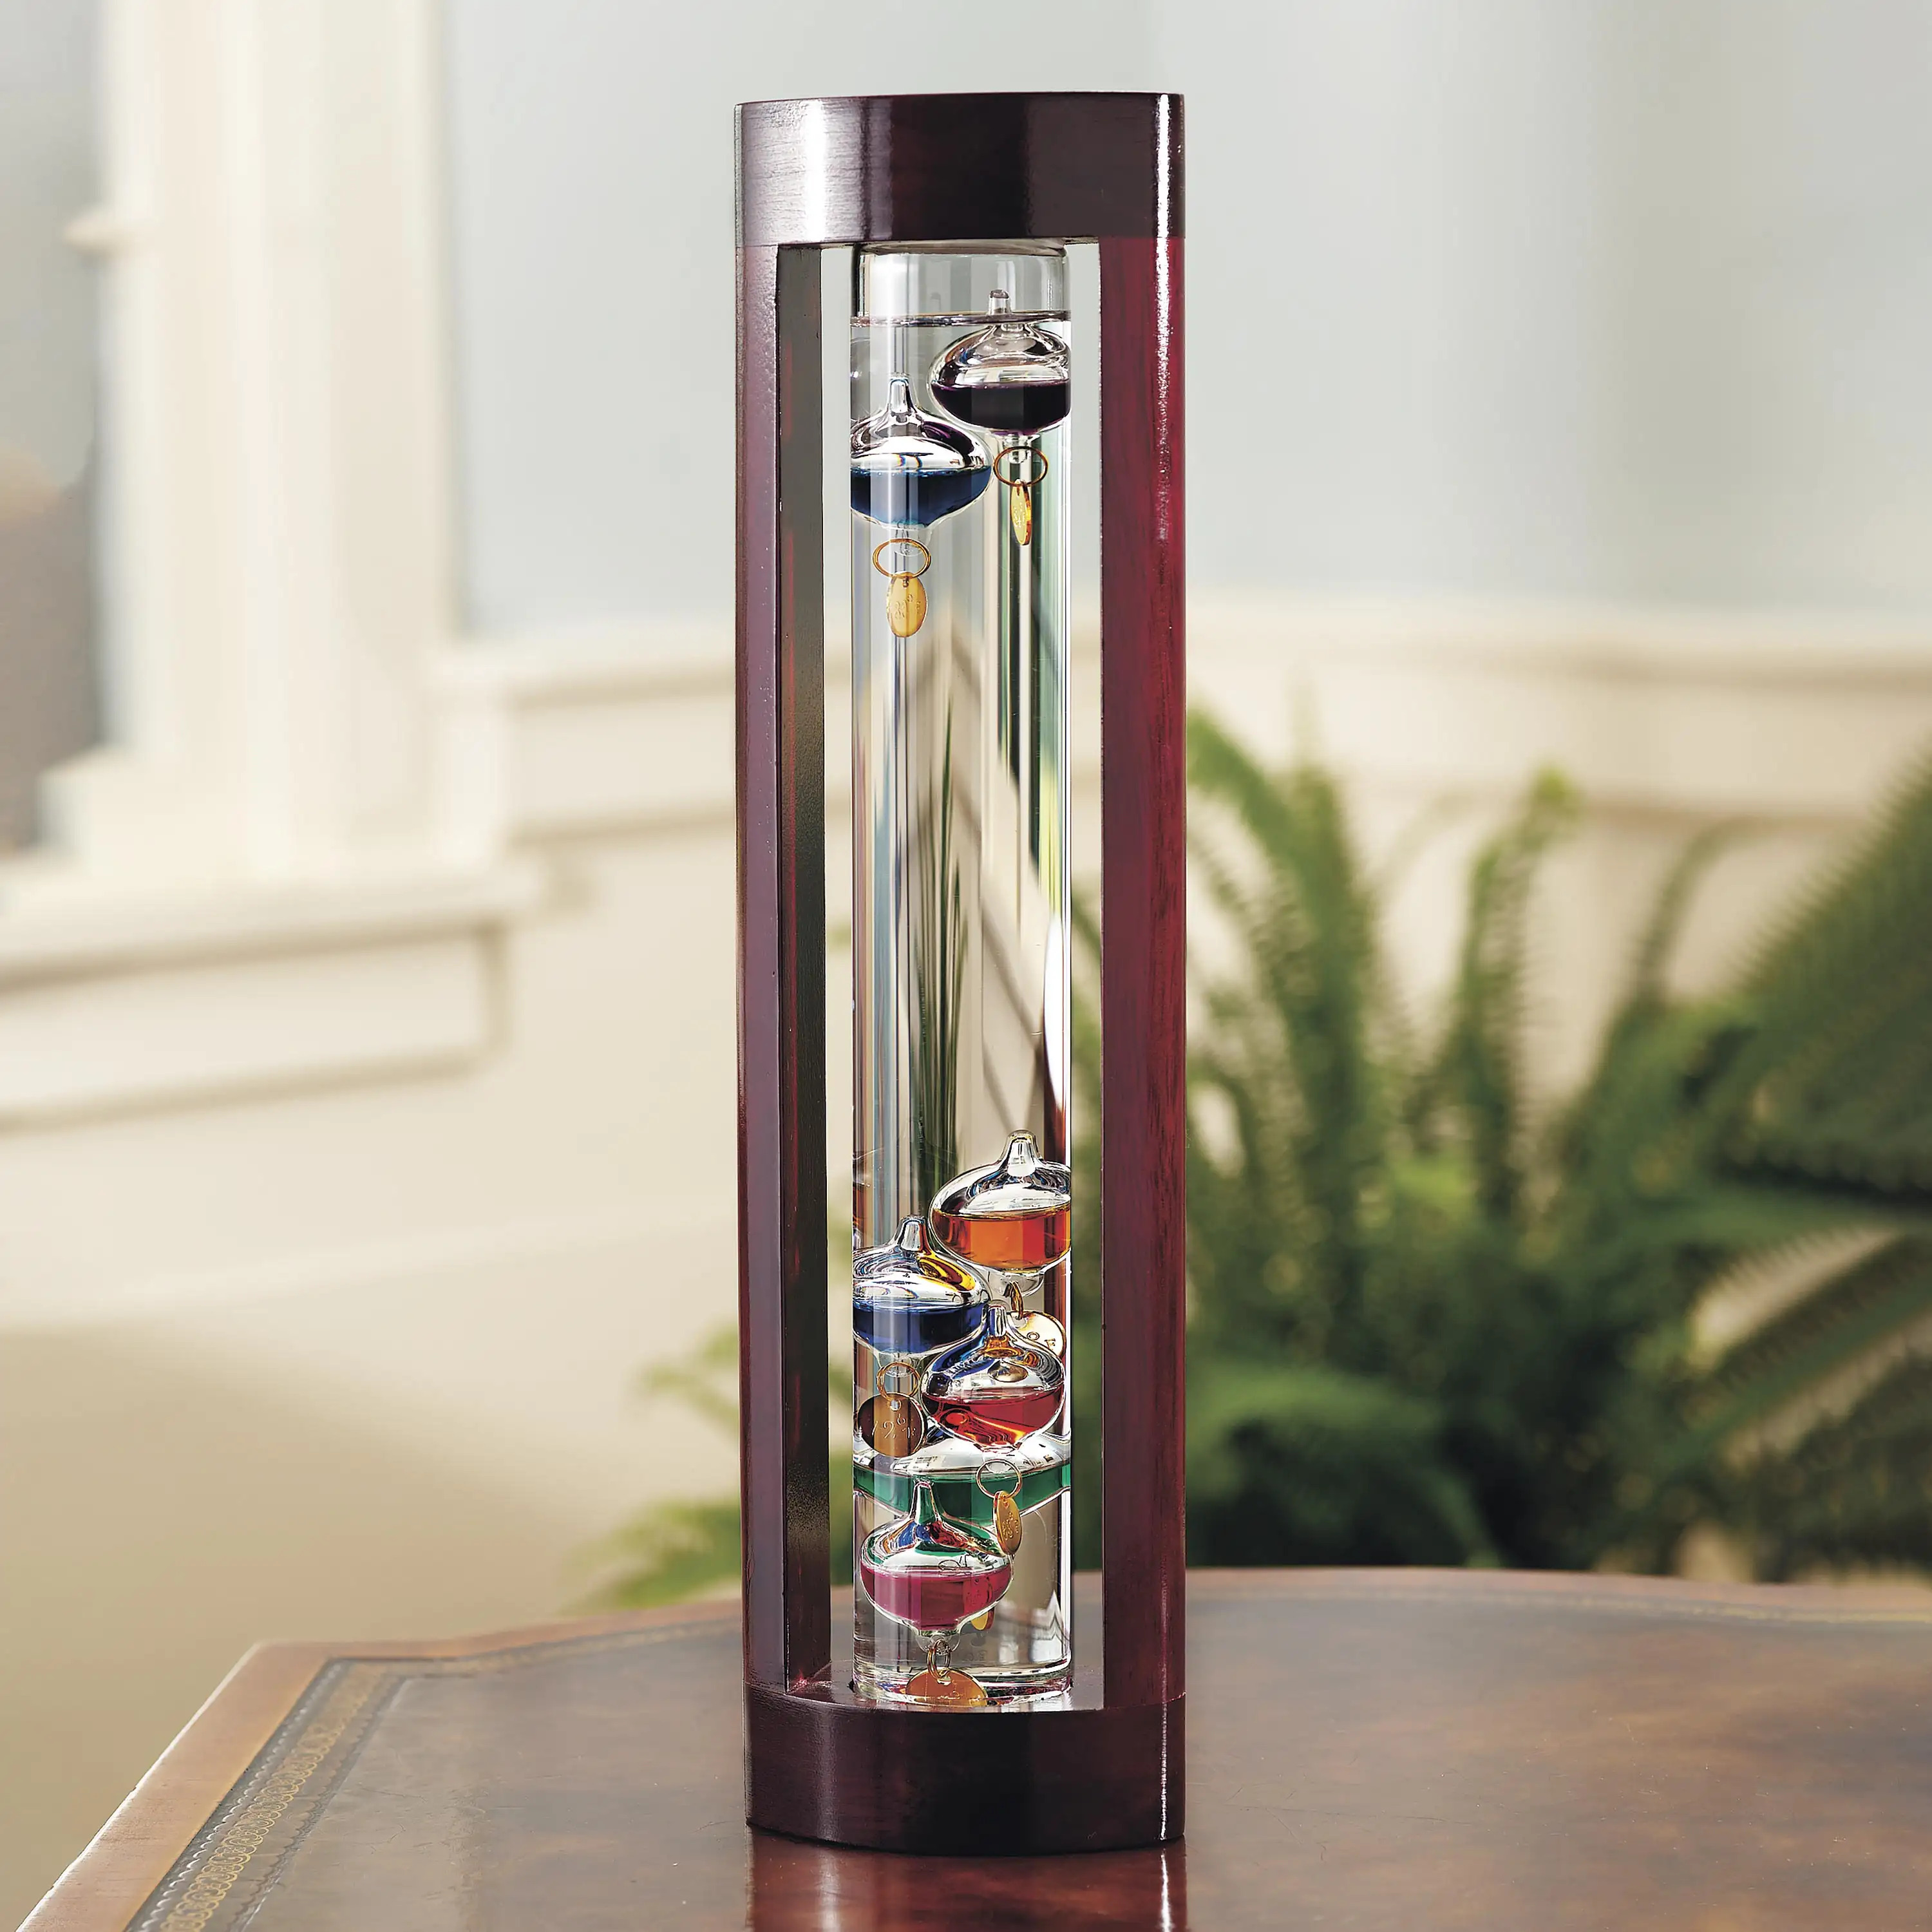
\includegraphics[width=0.7\textwidth,height=\textheight]{images/galileo-thermometer.jpg}
\caption[Galileo's Thermometer. The coloured balls are weighted
differently with tags that indicate temperature. They rise and fall as
the ambient temperature changes. This device, with changing bulb
positions, is the ideal metaphor for my idea of instantaneous caste, as
spelled out in this blog.]{Galileo's Thermometer. The coloured balls are
weighted differently with tags that indicate temperature. They rise and
fall as the ambient temperature changes. This device, with changing bulb
positions, is the ideal metaphor for my idea of instantaneous caste, as
spelled out in this blog.\footnotemark{}}\label{fig:galileo}
\end{figure}
\footnotetext{Image courtesy of ``Plow and Hearth'':
  \url{https://www.plowhearth.com/galileo-thermometer-with-cherry-finish-wood-frame/p/in6808}.}

\href{https://en.wikipedia.org/wiki/Galileo_thermometer}{Galileo's
Thermometer} is an ideal metaphor for my idea of caste. The device is
the same, but different temperatures result in different bulbs rising to
the top or falling to the bottom. The rising and falling of different
bulbs represents the changing caste of a person performing the same
action, even as his or her attitude to that action changes.

If you are intrigued by the Galileo Thermometer per se, you can see a
\href{https://youtube.com/shorts/kkQ1TFr4apg?si=V7W3fbIZLpQ2p4ud}{short
video here} {[}\citeproc{ref-galileo-YT-short}{1}{]} and a
\href{https://www.youtube.com/watch?v=XeSlFxOHW6A}{long video here}
{[}\citeproc{ref-galileo-YT-long}{2}{]}.

\subsubsection{Other viewpoints}\label{other-viewpoints}

My interpretation of caste in this blog has been wholly abstract,
philosophical, and spiritual. I consider caste as ever-changing, like a
\href{https://en.wikipedia.org/wiki/Quantum_fluctuation}{quantum
fluctuation}. Some might call such a view unrealistic or
\href{https://www.etymonline.com/search?q=Utopia}{Utopian}.

Caste is embedded in the social and economic fabric of contemporary
India at a very deep level. It has been tied to birth and to hereditary
occupation. Several eminent social thinkers do not see it as an evil,
but rather as the \href{https://en.wikipedia.org/wiki/Gluon}{gluon} that
has kept and still keeps Indian society together. Intellectuals like R
Vaidyanathan {[}\citeproc{ref-rv-caste}{3}{]} and Gurcharan Das
{[}\citeproc{ref-das-dharma}{4}{]} have examined caste from a broader
perspective, and the interested reader is referred to works such as
theirs for a different---and more pragmatic---take on caste in India.

\subsection{Acknowledgements}\label{acknowledgements}

I am grateful to ``Plow and Hearth'' for permission to use their
magnificent image of a Galileo's Thermometer in this blog.

\subsection{Feedback}\label{feedback}

Please \href{mailto:feedback.swanlotus@gmail.com}{email me} your
comments and corrections.

\noindent A PDF version of this article is
\href{./same-action-four-castes.pdf}{available for download here}:

\begin{small}

\begin{sffamily}

\url{https://swanlotus.netlify.app/blogs/same-action-four-castes.pdf}

\end{sffamily}

\end{small}

\section*{References}\label{bibliography}
\addcontentsline{toc}{section}{References}

\phantomsection\label{refs}
\begin{CSLReferences}{0}{0}
\bibitem[\citeproctext]{ref-galileo-YT-short}
\CSLLeftMargin{{[}1{]} }%
\CSLRightInline{Boba\_Queen88. 2023. {My Galileo Thermometer}. Retrieved
3 August 2024 from
\url{https://youtube.com/shorts/kkQ1TFr4apg?si=V7W3fbIZLpQ2p4ud}}

\bibitem[\citeproctext]{ref-galileo-YT-long}
\CSLLeftMargin{{[}2{]} }%
\CSLRightInline{Garry Eves. 2023. {What is a Galileo Thermometer and How
does it work?} Retrieved 3 August 2024 from
\url{https://www.youtube.com/watch?v=XeSlFxOHW6A}}

\bibitem[\citeproctext]{ref-rv-caste}
\CSLLeftMargin{{[}3{]} }%
\CSLRightInline{Vaidyanathan R. 2019. \emph{{Caste as Social Capital}}.
Westland.}

\bibitem[\citeproctext]{ref-das-dharma}
\CSLLeftMargin{{[}4{]} }%
\CSLRightInline{Gurcharan Das. 2012. \emph{{The Difficulty of Being
Good}: {On the Subtle Art of Dharma}}. Penguin.}

\end{CSLReferences}



\end{document}
